\section{ATM Straddle Strategy}\label{sec:5}

The straddle strategy sells approximately 30-day ATM straddles on underlyings with the lowest completed realized-minus-implied volatility (RV--IV) memories. The signal follows the volatility-premium motivation of Goyal and Saretto \cite{goyal2009}; our experiments evaluate entry sizing and capital allocation around this fixed trading rule.


\subsection{Trading Rules and Position Construction}

For every historical candidate, subtract entry ATM-call IV from the annualized RV measured after the next-session entry close through that contract's expiry. Only after the outcome finishes can it join the signal history. Average those completed RV - IV observations over the preceding 365 calendar days, requiring 126. Rank eligible names each day and sell the bottom 10\%.


\begin{equation*}M_{i,t}=\operatorname{mean}_{u:\,t-365<T_u<t}\left(RV_{i,u\to T_u}-IV^{\rm ATM\ call}_{i,u}\right).\end{equation*}

Selection uses the cross-sectional bottom decile of eligible completed-outcome memories, without an absolute volatility-gap threshold.



Each position sells an ATM call and put with the same underlying, strike and expiry, with daily stock-delta rebalancing. Full size targets \$450 combined call-and-put vega per IV point. The portfolio retains net short-gamma and short-vega exposure, including jump and volatility-revaluation risk.




The ranking uses ATM-call IV and annualized RV in volatility units, while execution uses the complete straddle. Profit is measured from the option-and-hedge ledger after costs and financing; the RV--IV ranking is neither a variance difference nor a profit identity.




\subsection{Ridge-Based Contexts}\label{sec:straddle-sizing}

The straddle sizing model fits a 60-month ridge model to completed full-size profit, using 14 inputs and requiring 128 examples. The inputs include IV, RV-IV memory, VIX and a separate fixed-half paper portfolio's recent performance. Score terciles define three contexts. Training uses only completed straddle outcomes and does not use the Q-allocation reward.

Training examples combine predetermined date-and-rank sampling of proposals with additional proposals admitted by a separate fixed-half benchmark portfolio. Only completed outcomes with finite reward labels enter fitting: 4,116 rewards are available in the saved sample. The fitted sizing policy is applied to all 35,774 proposals; future payoff availability does not restrict live proposals.

\subsection{Position-Size Selection}\label{sec:straddle-size-map}

Each context receives 50\%, 75\% or 100\% exposure. We enumerate all 27 context-to-size maps and retain the highest Sharpe on their aggregate completed daily straddle-profit paths, including overlapping positions. Insufficient history uses half size. The context-to-size map need not increase monotonically with the ridge score because selection maximizes completed-path Sharpe. Section~\ref{app:entry-optimization} provides exact fitting details. Feature-usage and admission diagnostics follow in Section~\ref{sec:straddle-results}.

\subsection{Results}\label{sec:straddle-results}

\subsubsection{Performance}

\begin{table}[H]\centering\small
\caption{Straddle entry-sizing policies in validation and later evaluation. S denotes annualized excess Sharpe; later profit is profit above cash.}\label{tab:straddle-entry-results}
\setlength{\tabcolsep}{4pt}\renewcommand{\arraystretch}{1.18}
\begin{tabularx}{\textwidth}{@{}>{\hsize=1.66992\hsize\linewidth=\hsize\raggedright\arraybackslash}X>{\hsize=0.81055\hsize\linewidth=\hsize\raggedleft\arraybackslash}X>{\hsize=0.81055\hsize\linewidth=\hsize\raggedleft\arraybackslash}X>{\hsize=0.73242\hsize\linewidth=\hsize\raggedleft\arraybackslash}X>{\hsize=0.97656\hsize\linewidth=\hsize\raggedleft\arraybackslash}X@{}}\toprule
\textbf{Entry policy} & \textbf{2018--21 S} & \textbf{2022--25 S} & \textbf{Later entries} & \textbf{Later profit}\\\midrule
Straddle \(\cdot\) 50\% & 0.740 & 0.920 & 1782 & \$1.824m\\
Straddle \(\cdot\) 75\% & 0.542 & 0.968 & 1222 & \$2.010m\\
Straddle \(\cdot\) 100\% & 0.528 & 0.990 & 940 & \$2.206m\\
Straddle \(\cdot\) Learned sizing & 0.775 & 1.041 & 1204 & \$2.379m\\
\bottomrule\end{tabularx}\end{table}

\begin{figure}[H]\centering
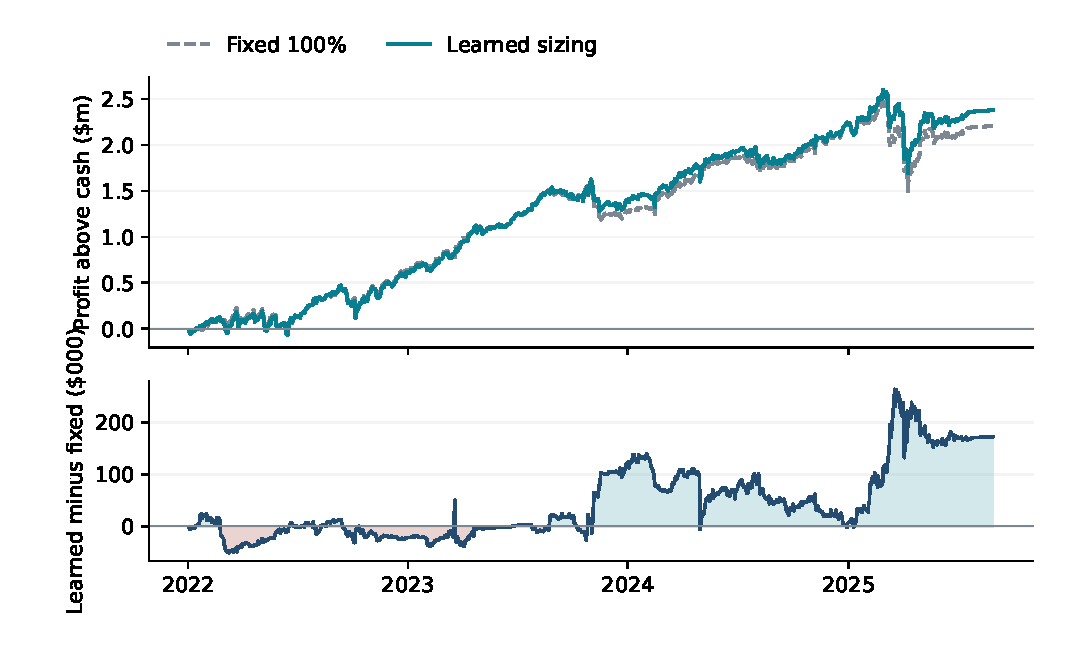
\includegraphics[width=\linewidth]{straddle_entry_curves.pdf}
\caption{Straddle profit above cash since January 2022. Top: learned and fixed-full entry sizing. Bottom: incremental profit, learned sizing minus fixed full sizing. Series subtract their 2021 closing values and retain carried positions. Differences reflect both sizing and admission.}\label{fig:straddle-entry-curves}
\end{figure}


The learned straddle sizing policy reaches Sharpe 1.041 and \$2.379 million above cash, compared with 0.990 and \$2.206 million at full size. Its earlier Sharpe also exceeds each fixed-size control.

As specified in Section~\ref{sec:evaluation-protocol}, all policies receive the same 35,774 straddle proposals, but size-dependent rounding, inventory and admission produce different funded entries. These comparisons measure complete sizing and admission policies rather than predictive sizing alone.

\subsubsection{Policy Interpretation and Trade Admission}

\begin{figure}[H]\centering
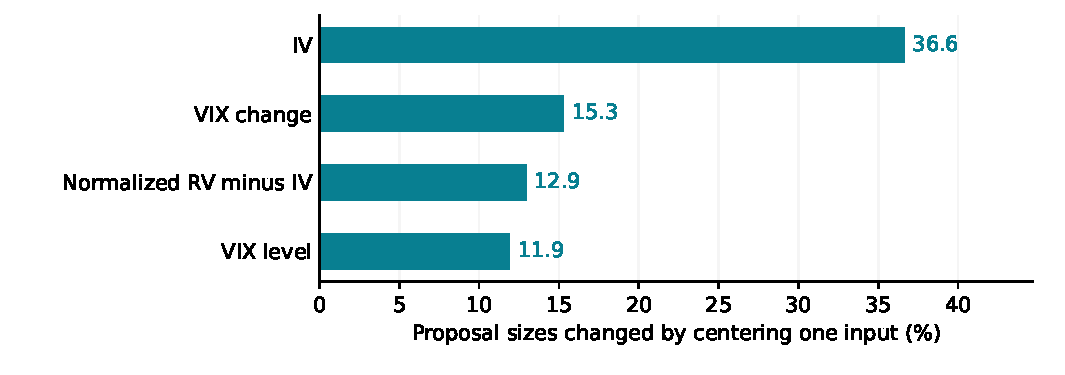
\includegraphics[width=\linewidth]{straddle_entry_explanations.pdf}
\caption{Straddle sizing sensitivity during later evaluation: the percentage of fitted proposal sizes that change when one input is centered. This descriptive sensitivity measure does not establish a causal effect on profit.}\label{fig:straddle-entry-explanations}
\end{figure}

For a straddle proposal, standardized ridge contributions add to a score. Saved thresholds locate its context, and the learned map selects a size. Centering IV changes 36.6\% of later fitted proposal sizes. Recent VIX change changes 15.3\%, normalized RV-minus-IV memory 12.9\%, and VIX level 11.9\%. The size map need not rise monotonically with the regression score because it optimizes the combined daily path. Exact replay reproduces every saved size across all 35,774 straddle proposals.

Later entry overlap with the fixed-full portfolio comprises 897 entries taken by both policies, 307 taken only by learned sizing and 43 taken only by fixed full size. These differences can arise through the inventory left by earlier size decisions. An explanation of proposed size alone therefore does not explain the entire portfolio result.

Among quote-available completed straddle labels, full-size profit averages \$1,631 for proposals assigned full size and \$16 for those assigned half size. This deliberately sampled subset also reflects admission by the fixed-half benchmark and finite-label availability; it is not a representative sample of all proposals. Three within-date size shuffles yield later Sharpes 0.834, 0.928 and 1.044, versus 1.041 learned. One shuffle exceeds the learned policy, so the funded results and feature-usage diagnostics alone do not establish predictive sizing.

Completed-cohort attribution is consistent with collecting a premium for movement risk. For both more persistent and more reversing price paths, aggregate option-plus-hedge profit is positive when entry straddle IV exceeds subsequent RV and negative when it does not. These groups use realized outcomes and are not available entry screens. There are 220 losing cohorts even when entry IV exceeds subsequent RV. Option and stock-hedge profits must be read together; positive hedge profit is not an independent trading edge. Appendix~\ref{app:h} retains the full-history attribution, IV--RV definitions and accounting reconciliation.

Joint sizing-and-allocation results follow in Section~\ref{sec:results}.
\FloatBarrier
